\documentclass[10pt]{book}
\usepackage{gvv-book}
\usepackage{gvv}
\usepackage[sectionbib,authoryear]{natbib}% for name-date citation comment the below line
\usepackage{setspace}
\setstretch{1.0}
%\usepackage[sectionbib,numbers]{natbib}% for numbered citation comment the above line
%%********************************************************************%%
%%       How many levels of section head would you like numbered?     %%
%% 0= no section numbers, 1= section, 2= section, 3= subsection %%
\setcounter{secnumdepth}{3}
%%********************************************************************%%
%%**********************************************************************%%
%%     How many levels of section head would you like to appear in the  %%
%%				Table of Contents?			%%
%% 0= chapter, 1= section, 2= section, 3= subsection titles.	%%
\setcounter{tocdepth}{2}
%%**********************************************************************%%
%\includeonly{ch01}
\makeindex
\let\cleardoublepage\clearpage
\begin{document}
\frontmatter
%%%%%%%%%%%%%%%%%%%%%%%%%%%%%%%%%%%%%%%%%%%%%%%%%%%%%%%%%%%%%%%%
\booktitle{Geometry}
\subtitle{Through Algebra}
\AuAff{Errala Paulsonashish}
%\halftitlepage
\titlepage
\tableofcontents
%\listoffigures %optional
%\listoftables  %optional
%% or Contributor Page for edited books
%% before \tableofcontents
%%%%%%%%%%%%%%%%%%%%%%%%%%%%%%%%%%%%%%%%%%%%%%%%%%%%%%%%%%%%%%%%
\setcounter{page}{0}
\begin{introduction}
This book shows how to solve problems in geometry using trigonometry and coordinate geometry. 
\end{introduction}
\mainmatter
\chapter{Triangle}
Consider a triangle with vertices
		\begin{align}
			\label{eq:tri-pts}
			\vec{A} = \myvec{-5 \\ -4},\,
			\vec{B} = \myvec{3 \\ -3},\,
			\vec{C} = \myvec{4 \\ 0}
		\end{align}
\section{Matrix}
The matrix of vertices of the triangle is defined as
		\begin{align}
			\vec{P} &= \myvec{\vec{A} & \vec{B} &\vec{C}} \\
            &=\myvec{-5 & 3 & 4 \\ -4 & -3 & 0}
		\end{align}
\begin{figure}[H]
    \centering
    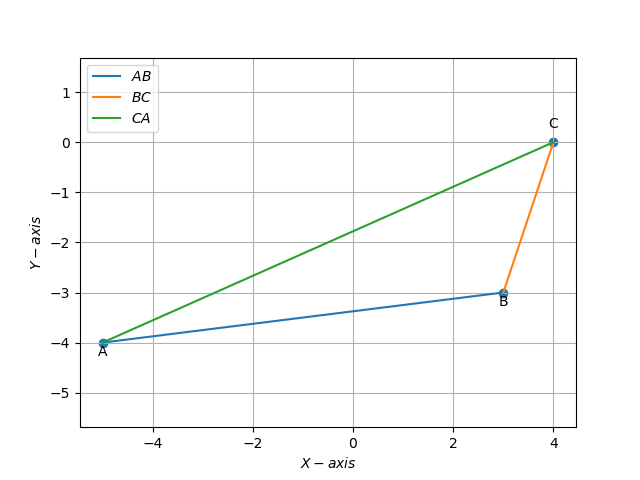
\includegraphics{figs/ABC_plot.png}
    \caption{$\triangle$ ABC}
    \label{fig:ABC_plot}
\end{figure}

\subsection{Vectors}
\begin{enumerate}[label=\thesubsection.\arabic*.,ref=\thesubsection.\theenumi]
\numberwithin{equation}{enumi}
%Question 1.6.1.1
\item Obtain the direction matrix of the sides of $\triangle \vec{ABC}$ defined as 
\begin{align}
\vec{M} = 	\myvec{\vec{A}-\vec{B} & \vec{B}-\vec{C} & \vec{C}-\vec{A}}
\end{align}
\\
\solution 
\begin{align}
\vec{M} &= \myvec{\vec{A}-\vec{B} & \vec{B}-\vec{C} & \vec{C}-\vec{A}} \\
	&= \myvec{\vec{A} & \vec{B} &\vec{C}} \myvec{1 & 0 & -1 \\ -1 & 1 & 0 \\ 0 & -1 & 1} \\
 &=\myvec{-5 & 3 & 4 \\ -4 & -3 & 0}\myvec{1 & 0 & -1 \\ -1 & 1 & 0 \\ 0 & -1 & 1} 
 \end{align}
 Using Matrix multiplication 
 \begin{align}
 \vec{M} &=\myvec{-8 & -1 & 9 \\ -1 & -3 & 4}
\end{align}
where the second matrix above is known as a {\em circulant} matrix.  Note that the $2^{nd}$ and $3^{rd}$ row of the above matrix are circular shifts of the $1^{st}$ row.
%Question 1.6.1.2
\item Obtain the normal matrix  of the sides of $\triangle \vec{ABC}$ \\
\solution\\
Considering the rotation matrix
\begin{align}
\vec{R} &= \myvec{0 & -1 \\ 1 & 0},
\end{align}
the normal matrix is obtained as
\begin{align}
\vec{N} &= \vec{R}\vec{M} \\
&=\myvec{0 & -1 \\ 1 & 0}\myvec{-8 & -1 & 9 \\ -1 & -3 & 4} 
\end{align}
Using matrix multiplication 
\begin{align}
   \vec{N} &= \myvec{1 & 3 & -4 \\ -8 & -1 & 9}
\end{align}
%Question 1.6.1.3
\item Obtain $\vec{a}, \vec{b}, \vec{c}$. \\
\solution \\
The sides vector is obtained as
\begin{align}
\vec{d} &= \sqrt{\text{diag}(\vec{M}^{\top}\vec{M})}\\
\vec{M}^{\top}\vec{M} &= \myvec{-8 &-1 \\ -1 &-3 \\ 9 &4}\myvec{-8 & -1 & 9 \\ -1 & -3 & 4}
\end{align} 
Using matrix multiplication 
\begin{align}
    \vec{M}^{\top}\vec{M} &= \myvec{ 65 & 11 & -76 \\ 11 & 10 & -21 \\ -76 & -21 & 97} \\
    \vec{d} &= \sqrt{\text{diag}\brak{\myvec{ 65 & 11 & -76 \\ 11 & 10 & -21 \\ -76 & -21 & 97}}} \\
    &= \myvec{ \sqrt{65} & \sqrt{10} & \sqrt{97}}
\end{align}
%Question 1.6.1.4
\item Obtain the constant terms in the equations of the sides of the triangle.\\
\solution \\The constants for the lines can be expressed in vector form as
\begin{align}
\vec{c} &= \text{diag}\cbrak{\brak{\vec{N}^{\top}\vec{P}}}  \\
\vec{N}^{\top}\vec{P} &= \myvec{1&-8 \\ 3&-1 \\ -4 &9}\myvec{-5 & 3 & 4 \\ -4 & -3 & 0} \\
\end{align}
Using matrix multiplication
\begin{align}
    &=\myvec{ 27 & 27 & 4 \\ -11 & 12 & 12 \\ -16 & -39 & -16 } \\
    \vec{c} &= \text{diag}\brak{ \myvec{ 27 & 27 & 4 \\ -11 & 12 & 12 \\ -16 & -39 & -16 }} \\
    &= \myvec{ 27 & 12 & -16}
\end{align}
\end{enumerate}


\subsection{Median}
\begin{enumerate}[label=\thesubsection.\arabic*.,ref=\thesubsection.\theenumi]
\numberwithin{equation}{enumi}
%Question 1.6.2.1
\item Obtain the midpoint matrix for the sides of the triangle \\
\solution
\begin{align}
\myvec{\vec{D} & \vec{E} &\vec{F}} &= \frac{1}{2}\myvec{\vec{A} & \vec{B} &\vec{C}}
\myvec{0 & 1 & 1 \\ 1 & 0 & 1 \\ 1 & 1 & 0} \\
&= \frac{1}{2}\myvec{-5 & 3 & 4 \\ -4 & -3 & 0}\myvec{0 & 1 & 1 \\ 1 & 0 & 1 \\ 1 & 1 & 0}
\end{align}
Using matrix multiplication 
\begin{align}
    \myvec{\vec{D} & \vec{E} &\vec{F}} &= \myvec{\frac{7}{2} & -\frac{1}{2} & -1 \\ -\frac{3}{2} & -2 & -\frac{7}{2}}
\end{align}
\begin{figure}[H]
    \centering
   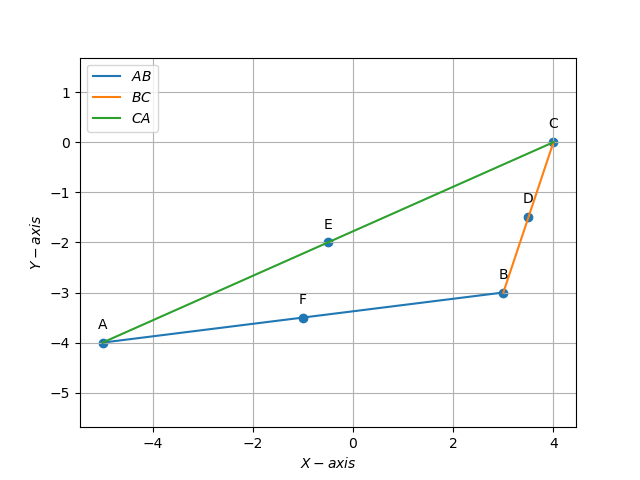
\includegraphics{figs/DEF_midpoints.png}
    \caption{mid-points}
    \label{fig:DEF_midpoints}
\end{figure}
%Question 1.6.2.2
\item Obtain the median direction matrix. \\
\solution \\
The median direction matrix is given by 
\begin{align}
			\vec{M}_1 &= \myvec{\vec{A}-\vec{D} & \vec{B}-\vec{E} & \vec{C}-\vec{F}}
			\\
			&= 
			  \myvec{
				  \vec{A}-\frac{\vec{B}+\vec{C}}{2} &
			  \vec{B}-\frac{\vec{C}+\vec{A}}{2} &
			  \vec{C}-\frac{\vec{A}+\vec{B}}{2}} 
			  \\
			  &= \myvec{\vec{A} & \vec{B} &\vec{C}}
			  \myvec{
				  1 & -\frac{1}{2} & -\frac{1}{2}
				  \\
				  -\frac{1}{2} & 1 & -\frac{1}{2}
				  \\
				  -\frac{1}{2} & -\frac{1}{2} & 1
				  } 
      \\
      &= \myvec{-5 & 3 & 4 \\ -4 & -3 & 0}\myvec{
				  1 & -\frac{1}{2} & -\frac{1}{2}
				  \\
				  -\frac{1}{2} & 1 & -\frac{1}{2}
				  \\
				  -\frac{1}{2} & -\frac{1}{2} & 1
				  } 
		\end{align}
  Using matrix multiplication 
  \begin{align}
   \vec{M}_1 &=   \myvec{-\frac{17}{2} & \frac{7}{2} & 5 \\ -\frac{5}{2} & -1 & \frac{7}{2}}
  \end{align}
%Question 1.6.2.3
\item Obtain the median normal matrix. \\
\solution \\
Considering the rotation matrix
\begin{align}
\vec{R}  = \myvec{0 & -1 \\ 1 & 0},
\end{align}
the normal matrix is obtained as
\begin{align}
\vec{N}_1 &= \vec{R}\vec{M}_1  \\
&=\myvec{0 & -1 \\ 1 & 0} \myvec{-\frac{17}{2} & \frac{7}{2} & 5 \\ -\frac{5}{2} & -1 & \frac{7}{2}} \\
\vec{N}_1 &=  \myvec{ \frac{5}{2} & 1 & -\frac{7}{2} \\ -\frac{17}{2} & \frac{7}{2} & 5 }
\end{align}
%Question 1.6.2.4
\item Obtain the median equation constants.
\begin{align}
\vec{c}_1 &= \text{diag}\brak{\brak{\vec{N}_1^{\top}\myvec{\vec{D} & \vec{E} & \vec{F} }}}  \\
\vec{N}_1^{\top}\myvec{\vec{D} & \vec{E} & \vec{F} } &= \myvec{\frac{5}{2}&-\frac{17}{2} \\ 1&\frac{7}{2} \\ -\frac{7}{2} &5}\myvec{\frac{7}{2} & -\frac{1}{2} & -1 \\ -\frac{3}{2} & -2 & -\frac{7}{2}}
\end{align}
Using matrix multiplication
\begin{align}
    &=\myvec{ \frac{43}{2} & \frac{63}{4} & \frac{109}{4} \\ -\frac{7}{4} & -\frac{15}{2} & -\frac{53}{4} \\ -\frac{79}{4} & -\frac{33}{4} & -14 } \\
    \vec{c}_1 &= \text{diag}\brak{ \myvec{ \frac{43}{2} & \frac{63}{4} & \frac{109}{4} \\ -\frac{7}{4} & -\frac{15}{2} & -\frac{53}{4} \\ -\frac{79}{4} & -\frac{33}{4} & -14 }} \\
    \vec{c}_1 &= \myvec{ \frac{43}{2} & -\frac{15}{2} & -14}
\end{align}
%Question 1.6.2.5
\item Obtain the centroid by finding the intersection of the medians.\\
\solution
 \begin{align}
\augvec{1}{1}{\vec{N}_1^{\top}& \vec{c}^{\top}}  &= \augvec{2}{1}{ \frac{5}{2} & -\frac{17}{2} & \frac{43}{2} \\ 1 & \frac{7}{2} & -\frac{15}{2} \\ -\frac{7}{2} & 5 & -14} 
\end{align}
Using Gauss-Elimination method:
\begin{align}
\augvec{2}{1}{ \frac{5}{2} & -\frac{17}{2} & \frac{43}{2} \\ 1 & \frac{7}{2} & -\frac{15}{2} \\ -\frac{7}{2} & 5 & -14} 
\xleftrightarrow[]{R_1 \leftarrow \frac{2R_1}{5}}
\augvec{2}{1}{ 1 & -\frac{17}{5} & \frac{43}{5} \\ 1 & \frac{7}{2} & -\frac{15}{2} \\ -\frac{7}{2} & 5 & -14} 
\\
\xleftrightarrow[]{R_2\leftarrow R_2-R_1}
\augvec{2}{1}{ 1 & -\frac{17}{5} & \frac{43}{5} \\ 0 & \frac{69}{10} & -\frac{161}{10} \\ -\frac{7}{2} & 5 & -14} 
\\
\xleftrightarrow[]{R_3\leftarrow R_3+\frac{7R_1}{2}}
\augvec{2}{1}{ 1 & -\frac{17}{5} & \frac{43}{5} \\ 0 & \frac{69}{10} & -\frac{161}{10} \\ 0 & -\frac{69}{10} & \frac{161}{10}}
\\
\xleftrightarrow[]{R_2\leftarrow \frac{10R_2}{69}}
\augvec{2}{1}{ 1 & -\frac{17}{5} & \frac{43}{5} \\ 0 & 1 & \frac{-7}{3} \\ 0 & -\frac{69}{10} & \frac{161}{10}}
\\
\xleftrightarrow[]{R_1\leftarrow R_1+\frac{17R_2}{5}}
\augvec{2}{1}{ 1 & 0 & \frac{2}{3} \\ 0 & 1 & -\frac{7}{3} \\ 0 & -\frac{69}{10} & \frac{161}{10}} \\
\xleftrightarrow[]{R_3\leftarrow R_3+\frac{69R_2}{10}}
\augvec{2}{1}{ 1 & 0 & \frac{2}{3} \\ 0 & 1 & -\frac{7}{3} \\ 0 & 0 & 0}\\
 \text{Therefore } \vec{G}=\myvec { \frac{2}{3} \\ -\frac{7}{3}}
\end{align} 
\begin{figure}[H]
    \centering
    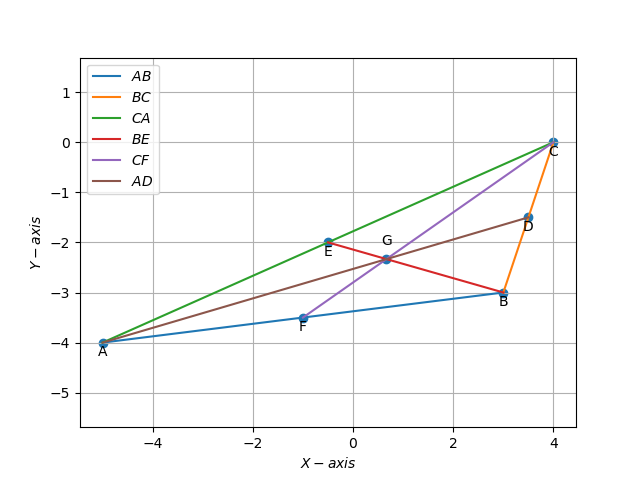
\includegraphics{figs/G_centroid.png}
    \caption{centroid of triangle ABC}
    \label{fig:mat_med2}
\end{figure}
\end{enumerate}

\subsection{Altitude}
\begin{enumerate}[label=\thesubsection.\arabic*.,ref=\thesubsection.\theenumi]
\numberwithin{equation}{enumi}
%Question 1.6.3.1
\item Find the normal matrix for the altitudes \\
\solution  The desired matrix is 
\begin{align}
\vec{M}_2 &= \myvec{\vec{B}-\vec{C} & \vec{C}-\vec{A} & \vec{A}-\vec{B} }
\\
&= 
\myvec{\vec{A} & \vec{B} &\vec{C}}
\myvec{ 0 & -1 & 1 \\ 1 & 0 & -1 \\ -1 & 1 & 0} \\
&= 
\myvec{-5 & 3 & 4 \\ -4 & -3 & 0}
\myvec{ 0 & -1 & 1 \\ 1 & 0 & -1 \\ -1 & 1 & 0}
\end{align}
Using Matrix multiplication 
\begin{align}
   \vec{M}_2 &=\myvec{-1 & 9 & -8 \\ -3 & 4 & -1}
\end{align}
%Question 1.6.3.2
\item Find the constant vector for the altitudes. \\
\solution\\
The desired vector is 
\begin{align}
\vec{c}_2 &= \text{diag}\cbrak{\brak{\vec{M}^{\top}\vec{P}}} \\
\vec{M}^{\top}\vec{P} &= \myvec{-1&-3 \\ 9&4 \\ -8 &-1}\myvec{-5 & 3 & 4 \\ -4 & -3 & 0} \\
\end{align}
Using matrix multiplication
\begin{align}
 \vec{M}^{\top}\vec{P}    &=\myvec{ 17 & 6 & -4 \\ -61 & 15 & 36 \\ 44 & -21 & -32 } \\
    \vec{c}_2 &= \text{diag}\brak{ \myvec{ 17 & 6 & -4 \\ -61 & 15 & 36 \\ 44 & -21 & -32 } } \\
 \vec{c}_2   &= \myvec{ 17 & 15 & -32}
\end{align}
\end{enumerate}
\begin{figure}[H]
    \centering
    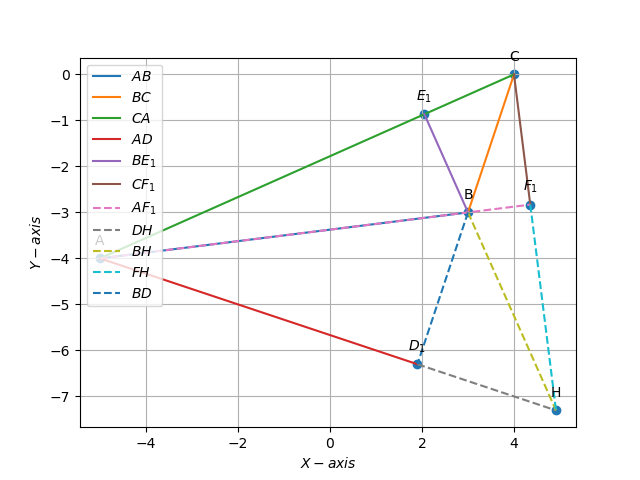
\includegraphics{figs/H_intersection.png}
    \caption{Orthocentre of $\triangle$ ABC}
    \label{fig:H_intersection}
\end{figure}


\subsection{Perpendicular Bisector}
\begin{enumerate}[label=\thesubsection.\arabic*.,ref=\thesubsection.\theenumi]
\numberwithin{equation}{enumi}
%Question 1.6.4.1
\item Find the normal matrix for the perpendicular bisectors \\
\solution\\
The normal matrix is $\vec{M}_2$
\begin{align}
       \vec{M}_2 &=\myvec{-1 & 9 & -8 \\ -3 & 4 & -1}
\end{align}
\begin{figure}[H]
    \centering
    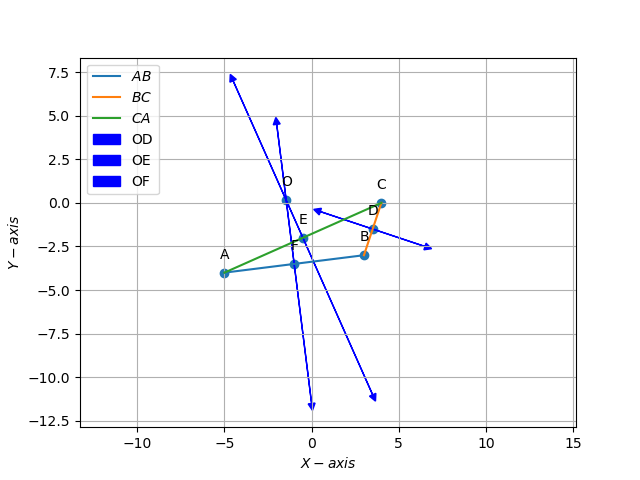
\includegraphics{figs/perpendicular_bisectors.png}
    \caption{plot of perpendicular bisectors}
    \label{fig:perpendicular_bisectors}
\end{figure}
%Question 1.6.4.2
\item Find the constants vector for the perpendicular bisectors. \\
\solution The desired vector is 
\begin{align}
\vec{c}_3 = \text{diag}\cbrak{\vec{M}_2^{\top}\myvec{\vec{D} & \vec{E} &\vec{F}}}
\end{align}
\solution
\begin{align}
\vec{c}_3 &= \text{diag}\cbrak{\vec{M}_2^{\top}\myvec{\vec{D} & \vec{E} &\vec{F}}} \\
\vec{M}_2^{\top}\myvec{\vec{D} & \vec{E} &\vec{F}} &= \myvec{-1&-3 \\ 9&4 \\ -8 &-1}\myvec{\frac{7}{2} & -\frac{1}{2} & -1 \\ -\frac{3}{2} & -2 & -\frac{7}{2}} \\
\end{align}
Using matrix multiplication
\begin{align}
 \vec{M}_2^{\top}\myvec{\vec{D} & \vec{E} &\vec{F}} &=\myvec{ 1 & \frac{13}{2} & \frac{23}{2} \\ \frac{51}{2} & -\frac{25}{2} & -23 \\ -\frac{5}{32} & 6 & \frac{23}{2} } \\
    \vec{c}_3 &= \text{diag}\brak{ \myvec{ 1 & \frac{13}{2} & \frac{23}{2} \\ \frac{51}{2} & -\frac{25}{2} & -23 \\ -\frac{5}{32} & 6 & \frac{23}{2} } } \\
 \vec{c}_3   &= \myvec{ 1 & -\frac{25}{2} & \frac{23}{2}}
\end{align}
\begin{figure}[H]
    \centering
     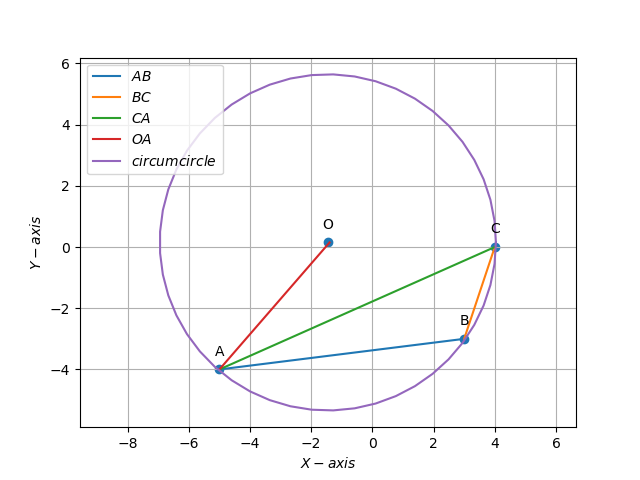
\includegraphics{figs/circumradius_o.png}
    \caption{circumcentre and circumcircle of $\triangle$ ABC}
    \label{fig:circumradius_o}
\end{figure}
\end{enumerate}
\subsection{Angle Bisector}
\begin{enumerate}[label=\thesubsection.\arabic*.,ref=\thesubsection.\theenumi]
\numberwithin{equation}{enumi}
%Question 1.6.5.1
\item Find the points of contact. \\ 
\solution\\
The points of contact are given by 
\begin{align}
\myvec{	\frac{n\vec{A}+p\vec{C}}{n+p}
&
\frac{p\vec{B}+m\vec{A}}{p+m}
&
\frac{m\vec{C}+n\vec{B}}{m+n}
}
= 	\myvec{\vec{A} & \vec{B} &\vec{C}}\myvec{\frac{n}{b} & \frac{m}{c} & 0\\0 & \frac{p}{c} & \frac{n}{a} \\\frac{p}{b} & 0 & \frac{m}{a}}
\end{align}
\begin{align}
    \myvec{\vec{p} & \vec{m} & \vec{n} } &=\frac{1}{2} \myvec{\vec{a} & \vec{b} & \vec{c}} \myvec{ -1 & 1 & 1 \\1 & -1 & 1 \\1 & 1 & -1 } \\
   &= \frac{1}{2}\myvec{ \sqrt{10}&  \sqrt{97} & \sqrt{65} }\myvec{ -1 & 1 & 1 \\1 & -1 & 1 \\1 & 1 & -1 }  \\
   &= \frac{1}{2}\myvec{ 3.16227766& 9.84885780 & 8.062257748 }\myvec{ -1 & 1 & 1 \\1 & -1 & 1 \\1 & 1 & -1 }
\end{align}
Using matrix multiplication 
\begin{align}
        \myvec{\vec{p} & \vec{m} & \vec{n} } &= \myvec{7.374418944& 0.687838804 & 2.474438856 }   \\
\myvec{\vec{A} & \vec{B} &\vec{C}}\myvec{\frac{n}{b} & \frac{m}{c} & 0\\0 & \frac{p}{c} & \frac{n}{a} \\\frac{p}{b} & 0 & \frac{m}{a}} 
  &= \myvec{-5 & 3 & 4 \\ -4 & -3 & 0} \myvec{\frac{2.474438856}{\sqrt{97}} & \frac{0.687838804 }{\sqrt{65}} & 0\\0 & \frac{7.374418944}{\sqrt{65}} & \frac{2.474438856}{\sqrt{10}} \\\frac{7.374418944}{\sqrt{97}} & 0 & \frac{0.687838804 }{\sqrt{10}}}
\end{align}
Using matrix multiplication We get the points of contact 
\begin{align}
    &= \myvec{ 1.7388292 & 2.31747277 & 3.21751372 \\ -1.0049648 & -3.0853159 & -2.34745882}
\end{align}
\begin{figure}[H]
    \centering
   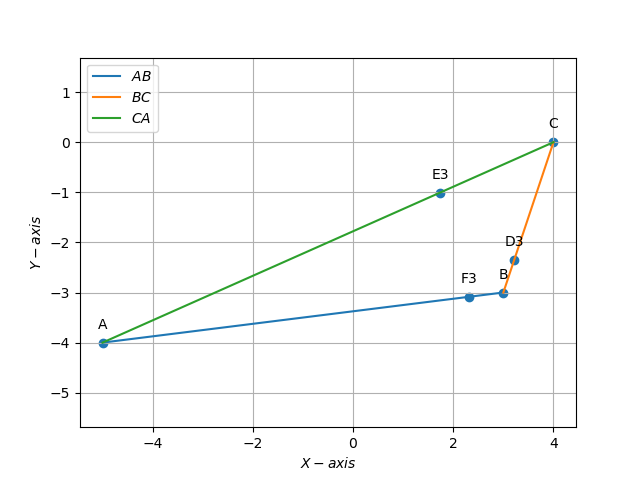
\includegraphics{figs/D3E3F3.png}
    \caption{Contact points of incircle of $triangle$ ABC}
    \label{fig:mat_ang1}
\end{figure}
\begin{figure}[H]
    \centering
    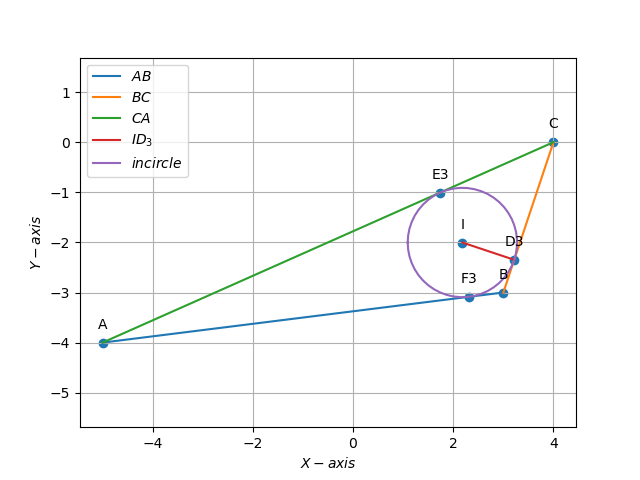
\includegraphics{figs/Incircle.png}
    \caption{Incircle and Incentre of $\triangle$ ABC }
    \label{fig:mat_ang2}
\end{figure}
\end{enumerate}
\end{document}
